\documentclass[12pt]{article}

\usepackage{../Ceyhun}

\begin{document}

	\hPage{ceyhun-201}

	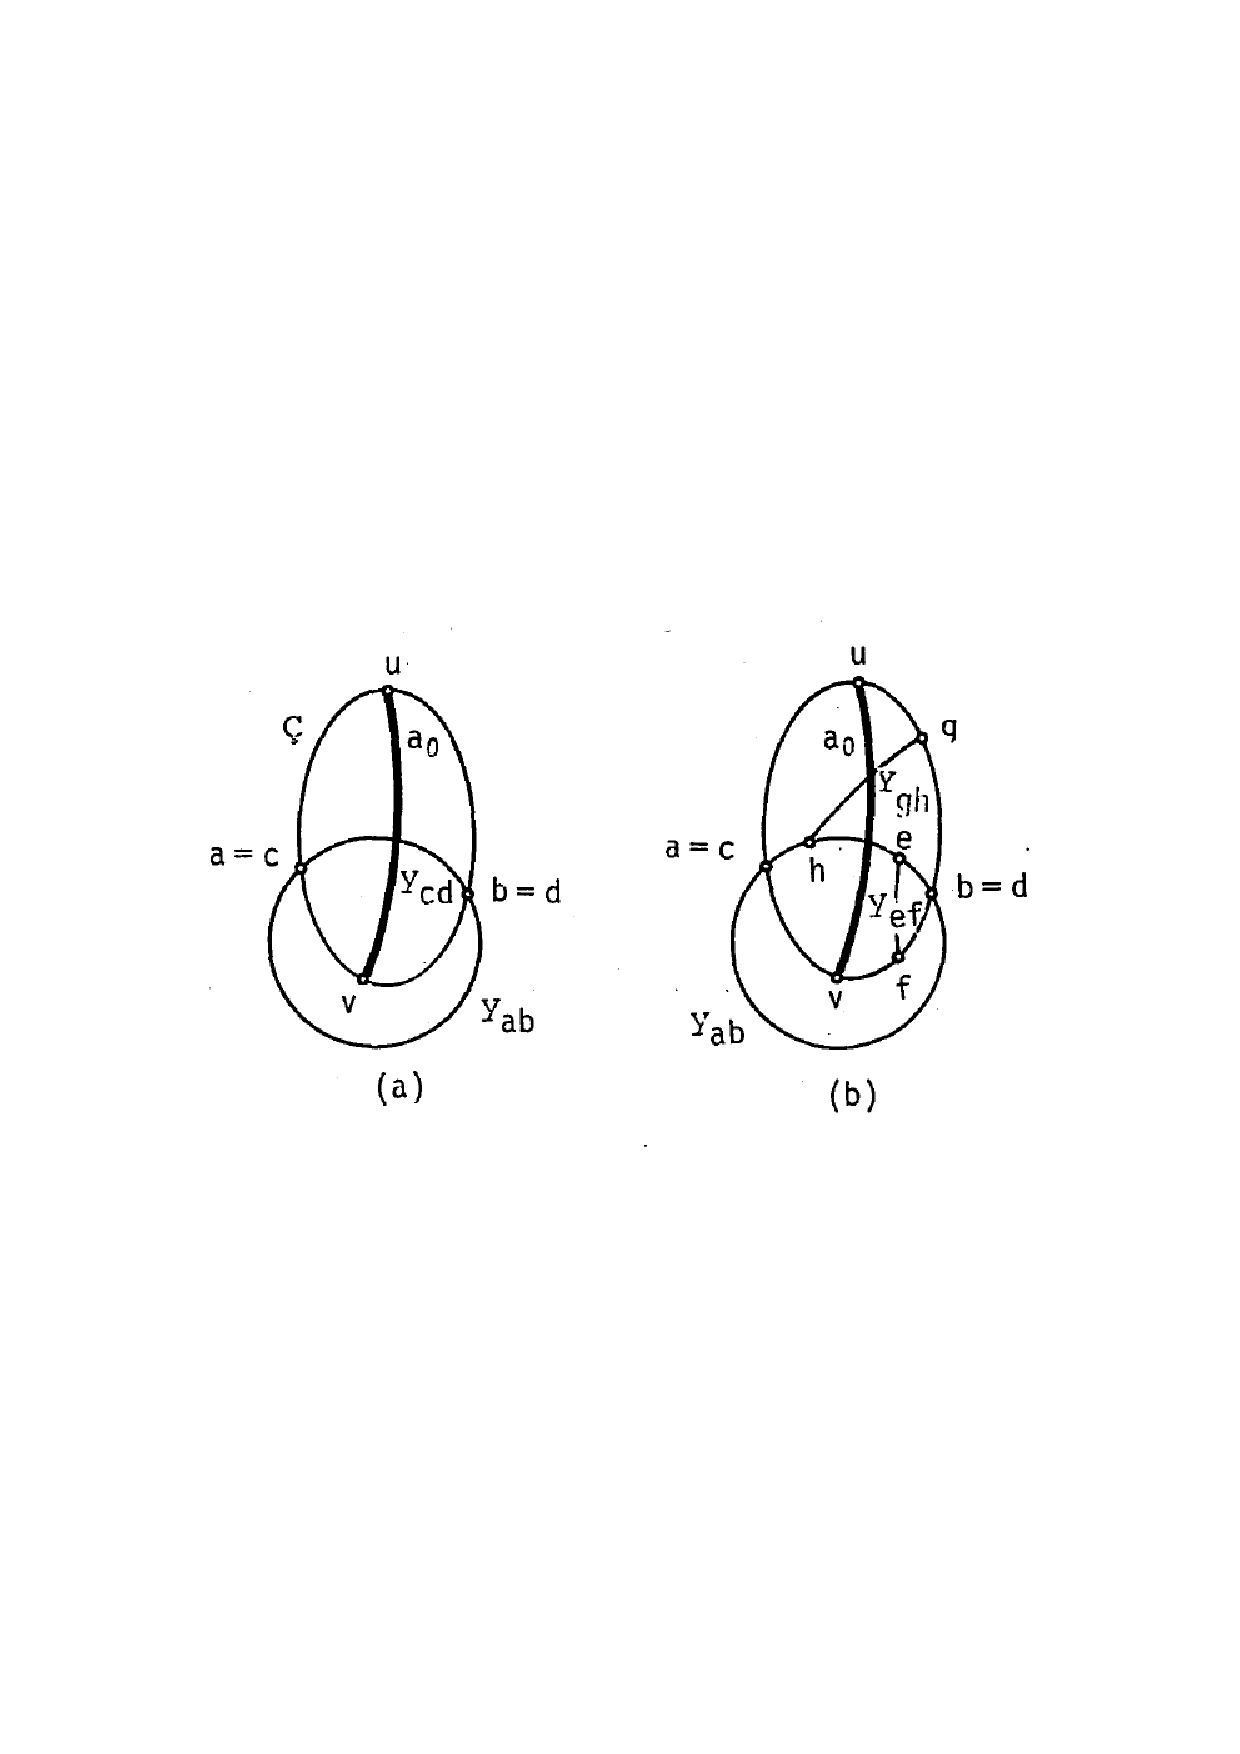
\includegraphics[trim={0 10cm 0 10cm},clip, width=0.8\textwidth]{images/ceyhun-201-fig01.pdf}

Şekil 4.2.4 Durum 3 ün incelenmesi.

bulunmalıdır. $Y_{gh}$ yolunun konumuna göre incelenmesi gerekli dört altdurum daha ortaya çıkmaktadır. Bunlardan, Şekil 4.2.5a, b ve c de gösterilenleri $K_{2}$, Şekil 4.2.5ç de gösterilen ise $K_{1}$ çizgesine kökteştir.

	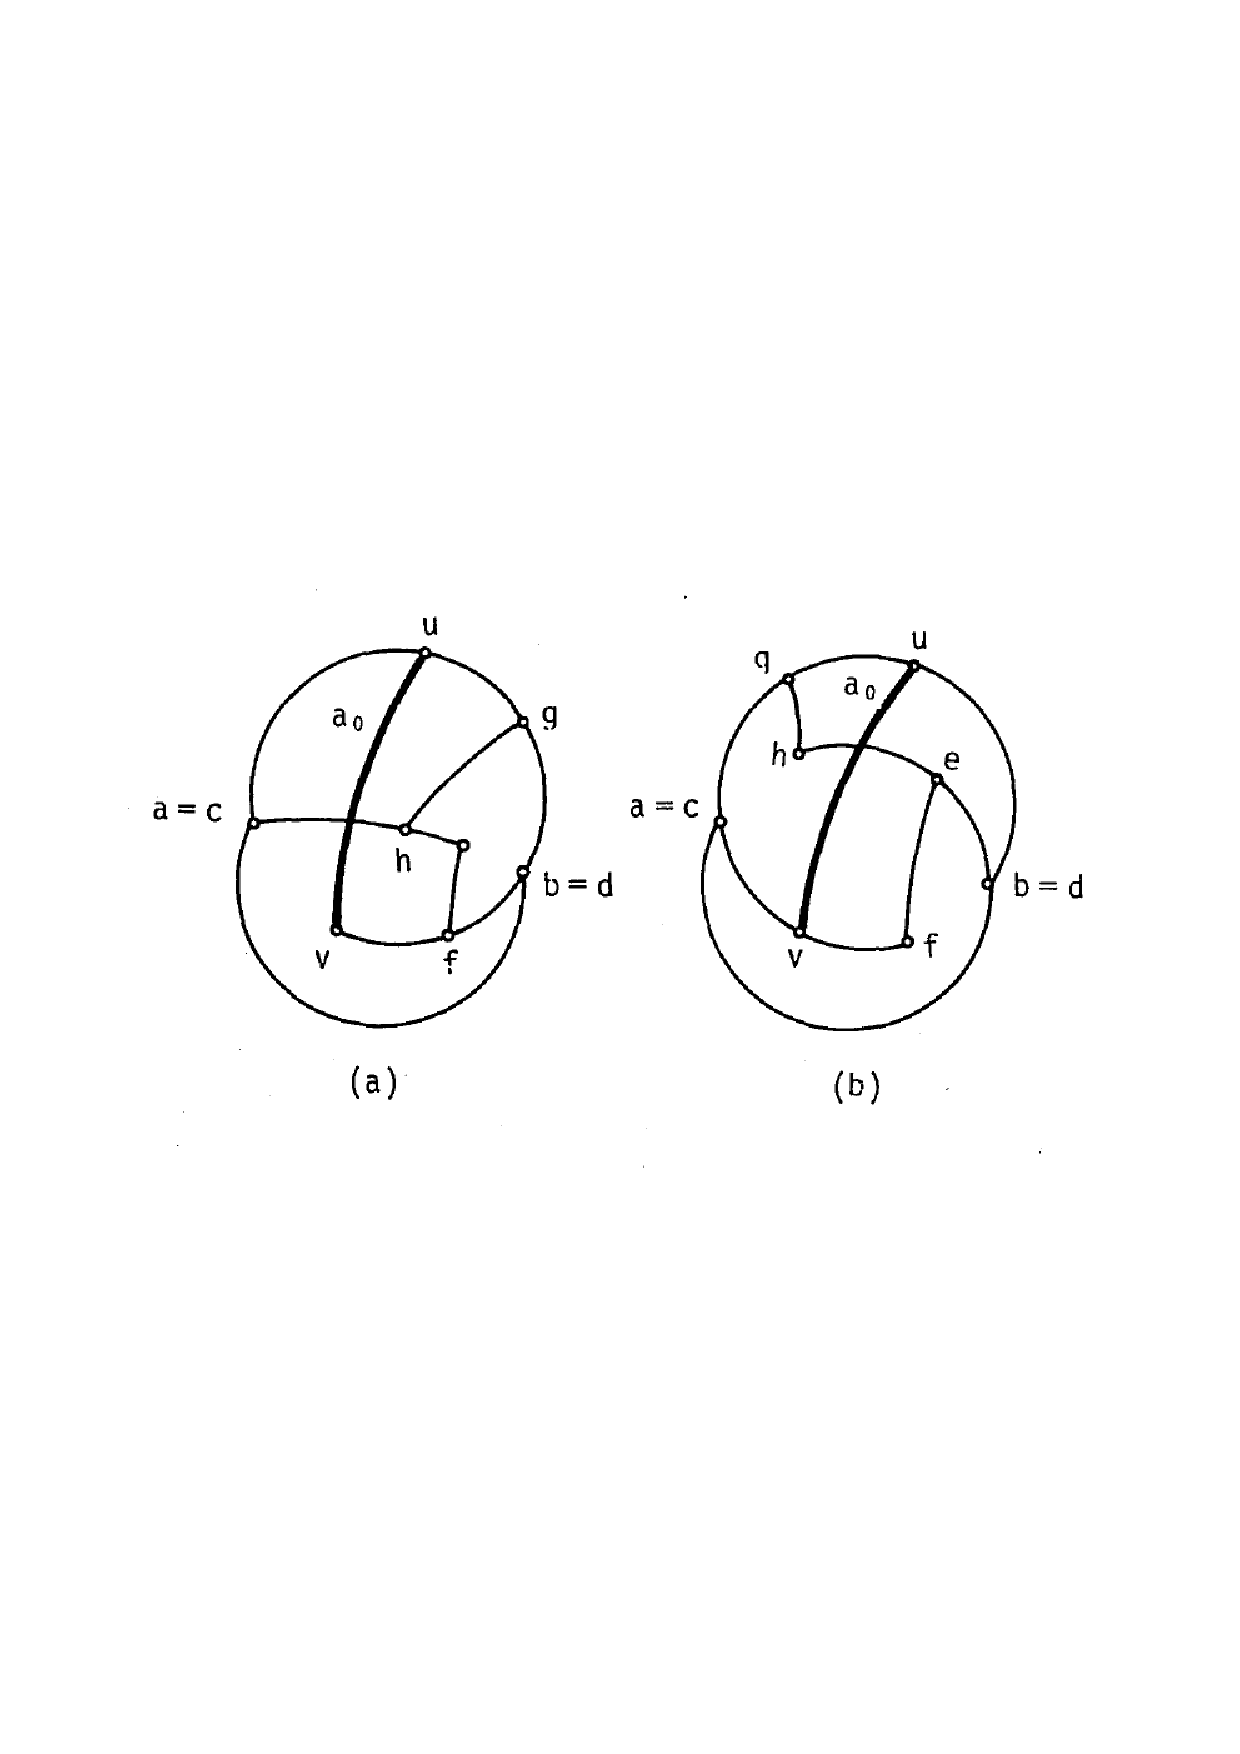
\includegraphics[trim={0 10cm 0 10cm},clip, width=0.8\textwidth]{images/ceyhun-201-fig02.pdf}

\end{document}